\documentclass[10pt]{article}
\usepackage[utf8]{inputenc}
\usepackage[english]{babel}
\usepackage[a4paper, margin=0.5cm]{geometry}
\usepackage{graphicx}
\usepackage{listings}
\usepackage{color}

\renewcommand{\familydefault}{\sfdefault}


\definecolor{mygreen}{rgb}{0,0.6,0}
\definecolor{mygray}{rgb}{0.5,0.5,0.5}
\definecolor{mymauve}{rgb}{0.58,0,0.82}

%\definecolor{grorange}{RGB}{224,110,47}
\definecolor{grorange}{RGB}{255,105,5}
\definecolor{grdarkorange}{RGB}{240,105,5}
%\definecolor{grgrey}{RGB}{114,112,111}
\definecolor{grgrey}{RGB}{125,125,125}
\definecolor{grlightgrey}{RGB}{239,239,239}

\lstset{ %
  backgroundcolor=\color{grlightgrey},   % choose the background color; you must add \usepackage{color} or \usepackage{xcolor}; should come as last argument
  basicstyle=\tiny,        % the size of the fonts that are used for the code
  breakatwhitespace=false,         % sets if automatic breaks should only happen at whitespace
  breaklines=true,                 % sets automatic line breaking
  postbreak=\raisebox{0ex}[0ex][0ex]{\ensuremath{\color{grdarkorange}\hookrightarrow\space}},
  captionpos=t,                    % sets the caption-position to bottom
  commentstyle=\color{grgrey},    % comment style
  deletekeywords={...},            % if you want to delete keywords from the given language
  escapeinside={\%*}{*)},          % if you want to add LaTeX within your code
  extendedchars=true,              % lets you use non-ASCII characters; for 8-bits encodings only, does not work with UTF-8
  frame=none,	                   % adds a frame around the code
  keepspaces=true,                 % keeps spaces in text, useful for keeping indentation of code (possibly needs columns=flexible)
  keywordstyle=\color{grorange},       % keyword style
  language=Python,                 % the language of the code
  morekeywords={*,...},           % if you want to add more keywords to the set
  numbers=none,                    % where to put the line-numbers; possible values are (none, left, right)
  numbersep=5pt,                   % how far the line-numbers are from the code
  numberstyle=\tiny\color{grgrey}, % the style that is used for the line-numbers
  rulecolor=\color{black},         % if not set, the frame-color may be changed on line-breaks within not-black text (e.g. comments (green here))
  showspaces=false,                % show spaces everywhere adding particular underscores; it overrides 'showstringspaces'
  showstringspaces=false,          % underline spaces within strings only
  showtabs=false,                  % show tabs within strings adding particular underscores
  stepnumber=2,                    % the step between two line-numbers. If it's 1, each line will be numbered
  stringstyle=\color{grdarkorange},     % string literal style
  tabsize=2,	                   % sets default tabsize to 2 spaces
  title=\lstname                   % show the filename of files included with \lstinputlisting; also try caption instead of title
}

\usepackage{multicol}

\begin{document}


\includegraphics[width=0.95\linewidth]{gnuradio_logo_web}


\begin{multicols*}{3}
\section{Installation}

\lstinputlisting[language=sh]{gnuradio-install.sh}


\section{Getting Started}

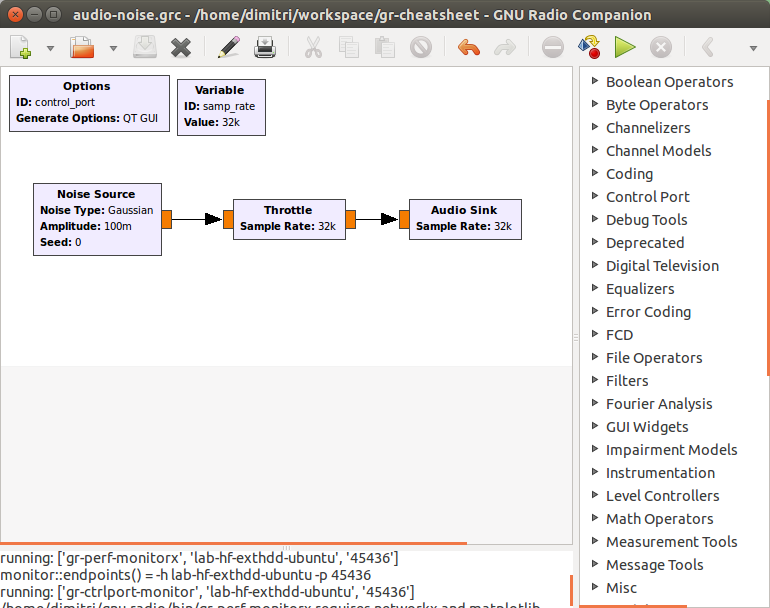
\includegraphics[width=0.99\linewidth]{./grc-screenshot}

\lstinputlisting[language=Python]{top_block.py}

\section{Gnu Radio Basics}

\subsection{Create Hierarchical Block}

\lstinputlisting[language=Python]{inputLayer.py}

\subsection{Create Python Block}

\lstinputlisting[language=Python]{vector_sum_vff.py}

%\subsection{Create C++ Block}
%
%\subsection{Streams and Vectors}
%
%\subsection{Stream Tags}
%
%\subsection{Message Passing}

\subsection{Post-Processing}

\lstinputlisting[language=Matlab]{read_binary_file.m}

\subsection{Performance Monitoring}

\lstinputlisting[language=sh]{gr-perf-monitorx-prerequiremets.sh}

\lstinputlisting[caption={./gnuradio/config.conf}]{config.conf}

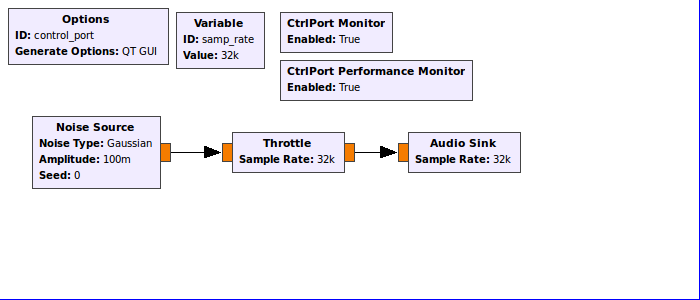
\includegraphics[width=0.99\linewidth]{control-port.png}

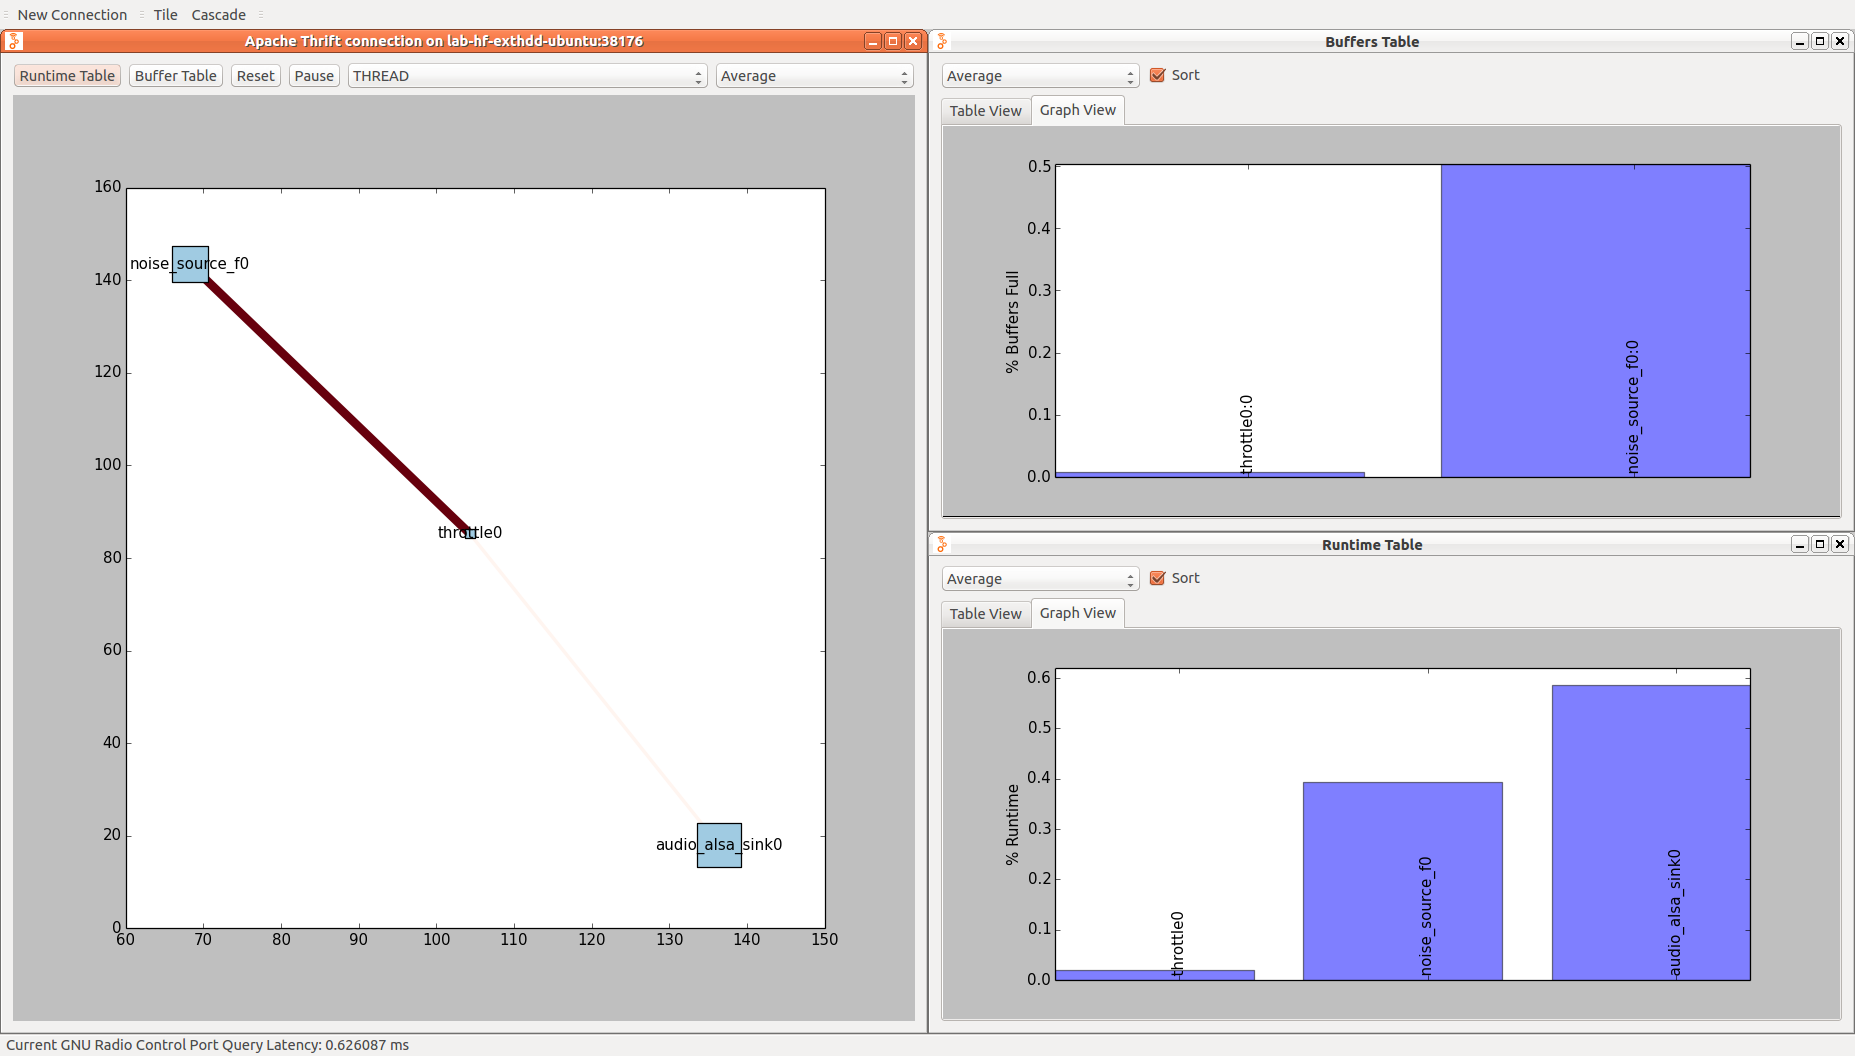
\includegraphics[width=0.99\linewidth]{gr-perf-monitorx-screenshot.png}

\begin{description}
\item[Block size] Processing time
\item[Edge color/width] Output buffer fullness
\end{description}


%\section{Signal Processing}
%
%\subsection{Channel Models}
%
%\subsection{Digital Modulation}
%
%\subsection{Filtering}
%
%\subsection{Resampling}
%
%\subsection{FFT}

\end{multicols*}
\end{document}